%% ===================================================================
%%  CSE 402 Final Project Report
%%  ACM sigconf template (non-anonymous, course submission)
%%  Build:  latexmk -pdf report.tex
%%
%%  TODO before submitting:
%%    - fill in Group number, Section, and student IDs (search "TODO")
%%    - put the three PNGs in ./fig/  (fig_waiting, fig_arrival, fig_staffing)
%%    - replace the GitHub URL in Section 4.1
%% ===================================================================
\documentclass[sigconf]{acmart}

\settopmatter{printacmref=false}
\renewcommand\footnotetextcopyrightpermission[1]{}
\pagestyle{plain}
\setcopyright{none}
\acmConference[CSE 402]{Final Project Report, January 2026 Term}{October 2026}{BUET, Dhaka, Bangladesh}

\usepackage{booktabs}
\usepackage{amsmath}
\usepackage{graphicx}
\usepackage{tikz}
\usetikzlibrary{arrows.meta, positioning, shapes.geometric, calc, fit, backgrounds}

\definecolor{c1}{HTML}{2A78D6}
\newcommand{\Wtot}{\overline{W}_{\text{total}}}

\begin{document}

\title{Congestion-Aware Diagnostic Routing in Emergency Departments:
A Discrete-Event Simulation Study}
\subtitle{CSE 402 Final Project Report --- Group 1, Section C}

\author{Shatabdi Dutta Chowdhury}
\affiliation{\institution{Student ID: 2105123}\city{}\country{}}
\email{shatabdi198dc@gmail.com}

\author{Arpita Dhar}
\affiliation{\institution{Student ID: 2105137}\city{}\country{}}
\email{arpitadhar436@gmail.com}

\author{Tasnimzaman Tanmi}
\affiliation{\institution{Student ID: 2105147}\city{}\country{}}
\email{tanmibuet@gmail.com}

\author{Fatin Ishrak Arian}
\affiliation{\institution{Student ID: 2105143}\city{}\country{}}
\email{fiarian1234@gmail.com}

\author{Shahir Bin Julfikar Aorko}
\affiliation{\institution{Student ID: 2105149}\city{}\country{}}
\email{aorko321@gmail.com}

\renewcommand{\shortauthors}{Chowdhury et al.}

\begin{abstract}
This project reproduces and extends the discrete-event emergency-department
(ED) scheduling model of Lv et al., which compares three physician-scheduling
policies but represents the diagnostic stage as a fixed examination sequence
without queues at individual testing stations. We first reimplemented their
model in Python and SimPy and verified that it reproduces their reported
physician and equipment utilization within half a percentage point. We then
extended the diagnostic stage by giving laboratory, CT, X-ray and ultrasound
their own single-server queues, letting each patient select the next required
examination from the current station workload, and counting the resulting
station queueing as patient waiting time. Over 100 paired replications,
congestion-aware routing reduces station queueing by $28.2\%$ but increases
total diagnostic-stage time by $5.0\%$, because station queueing accounts for
only $1.70\%$ of that stage while the discarded ordering had been overlapping
the reporting delays that dominate it. A four-way factorial comparison further
shows that the slack-based policy's tuned thresholds do not transfer between
the two diagnostic models: changing the routing rule alone costs $4.45$ min and
changing the thresholds alone $2.75$ min, whereas changing both costs only
$0.74$ min and is not significant. Sensitivity analysis over demand and
staffing shows that policy differences grow with load and vanish as physician
capacity increases.
\end{abstract}

\keywords{discrete-event simulation, emergency department, patient scheduling,
diagnostic routing, parameter transferability, SimPy}

\maketitle


\section{Introduction and Base Paper Review}
\label{sec:intro}

\subsection{Background}

Emergency departments (EDs) are systems in which patients, physicians and
diagnostic equipment interact continuously. When demand is high, limited
resources produce longer waits and poorer clinical outcomes~\cite{hoot2008crowding}.
Because controlled experiments in a live hospital are impractical,
discrete-event simulation (DES) is the standard tool for comparing ED
scheduling policies~\cite{gul2015review,vanbrabant2019review,saghafian2015review,
law2015simulation,banks2010des}.

The central scheduling question is which patient a physician should see next.
Policies may prioritize the most urgent patients, reserve capacity for patients
returning after diagnostic testing, or raise priority as a patient approaches a
clinical deadline~\cite{davenport2001slack}.

\subsection{The base paper}

Our base paper is Lv et al.~\cite{lv2026des}, \emph{Discrete Event
Simulation-Based Analysis and Optimization of Emergency Patient Scheduling
Strategies} (Healthcare, 2026). The paper builds a weekly DES model of a single
ED and compares three physician-scheduling policies.

\textbf{Model.} Patients arrive by a non-homogeneous Poisson process with
hourly rates estimated from one hospital's records, and are triaged as Level
III ($25\%$) or Level IV ($75\%$). Physicians are pooled by shift ($5$/$5$/$3$).
A patient receives an initial consultation, and with probability $0.60$ is sent
for diagnostic testing; the required subset of \{laboratory, CT, X-ray,
ultrasound\} is sampled independently with probabilities $0.92$, $0.55$, $0.29$
and $0.22$. Each examination has a processing time $\tau_j$ and a reporting
delay $\delta_j$ (Table~\ref{tab:params}). Once all results are available the
patient rejoins the queue for a follow-up consultation.

\textbf{Policies.} Three rules allocate physicians among Level III initial,
Level IV initial and follow-up patients: a fixed priority order (IFP), an
alternating split of capacity (ALT), and a slack-based policy (SBP) with two
tunable anticipation margins $(k_1,k_2)$ that the authors optimize by grid
search.

\textbf{Reported findings.} The authors report that SBP achieves the lowest
mean waiting time and conclude that it outperforms the alternatives.

\subsection{Gap addressed by this project}

Within the diagnostic stage, the base paper orders a patient's required tests
once, in descending order of reporting delay, and never revises that order.
Although the model adds a delay when equipment is occupied, it does not
represent a queue at each individual station, so the examination sequence
cannot respond to congestion the patient actually encounters. In a real
department a patient who finds the CT scanner busy would typically complete
another required test first.

\subsection{Objective and contributions}

The objective of this project is to reproduce the base model, extend its
diagnostic stage to a congestion-aware representation, and measure what that
added realism changes. Our contributions are:

\begin{enumerate}
\item A full reimplementation of the base model in Python/SimPy, validated
against the utilization figures reported in~\cite{lv2026des}.
\item A congestion-aware diagnostic stage: four single-server station queues
and a routing rule that selects each patient's next examination from the
current station workload.
\item An extended waiting-time metric that counts station queueing, which the
base paper's measure omits.
\item A quantitative finding that the routing rule reduces the quantity it
targets yet lengthens the diagnostic stage, together with the mechanism that
explains it.
\item A factorial experiment showing that the SBP thresholds and the diagnostic
routing rule cannot be tuned independently.
\end{enumerate}


\section{Methodology}
\label{sec:method}

For completeness the description below includes the components of the base
model~\cite{lv2026des} that we reimplemented, together with our modifications.
Unless stated otherwise, arrivals, triage, staffing, consultation-time
distributions, examination requirements, processing and reporting times, and
the three scheduling policies follow the base paper. Our extension is confined
to the diagnostic stage.

\subsection{System model}
\label{sec:system}

The system is a single ED with two triage classes, Level III and Level IV.
Figure~\ref{fig:flow} shows the patient flow. Patients arrive by a
non-homogeneous Poisson process with rate $\lambda_{d,h}$ varying by day $d$
and hour $h$ over a weekly cycle, using the hourly arrival data
of~\cite{lv2026des}. Each patient is Level III with probability $0.25$ and
Level IV with probability $0.75$. The waiting-time targets are $T_3=30$ min and
$T_4=120$ min; a patient is delayed when their waiting time exceeds the target.

Patients enter the initial-consultation queues and are selected by the
scheduling policy of Section~\ref{sec:scheduling}. The physician pool is $5$
(07:00--15:00), $5$ (15:00--22:00) and $3$ (22:00--07:00). Initial consultation
time is truncated exponential with mean $9$ min on $[5,15]$. With probability
$p_{\mathrm{exam}}=0.60$ the patient then requires diagnostic testing;
otherwise the patient is discharged.

The diagnostic subsystem contains four single-server stations, each with its
own queue. The required modalities are sampled independently with the
probabilities in Table~\ref{tab:params}; if the sampling yields no examination,
one modality is drawn uniformly.

\begin{figure*}[t]
\centering
\resizebox{\textwidth}{!}{%
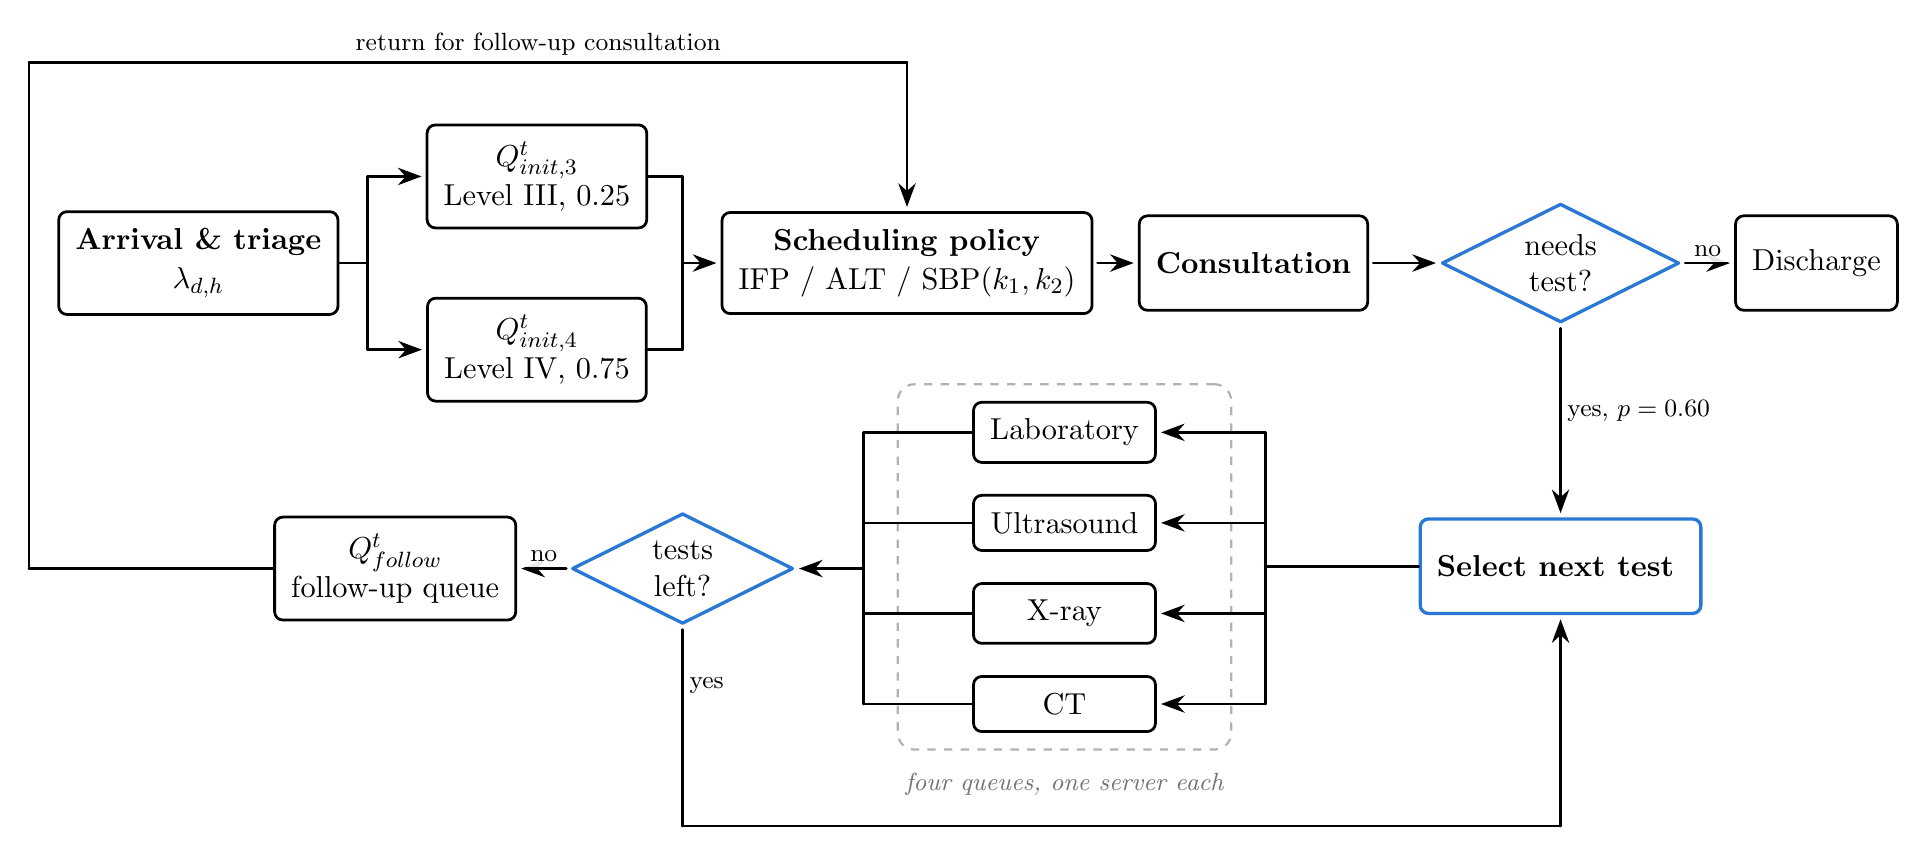
\begin{tikzpicture}[
  font=\fontsize{11}{13.2}\selectfont, x=1cm, y=1cm,
  line cap=round, line join=round,
  box/.style={draw=black, fill=white, rounded corners=3pt, line width=1.0pt,
              align=center, inner sep=6pt, minimum height=12mm},
  st/.style={box, text width=21mm, inner xsep=3pt, minimum height=7mm},
  dec/.style={draw=c1, fill=white, line width=1.2pt, align=center,
              inner sep=3pt, diamond, aspect=2.0},
  sel/.style={box, draw=c1, line width=1.2pt},
  fl/.style={-{Stealth[length=3.0mm,width=2.2mm]}, draw=black, line width=1.0pt,
              shorten >=1.5pt},
  fla/.style={fl, shorten <=1.5pt},
  ln/.style={draw=black, line width=1.0pt},
  lb/.style={font=\fontsize{9.5}{11}\selectfont, inner sep=2pt,
             fill=white, fill opacity=0.9, text opacity=1},
  grp/.style={draw=black!30, line width=0.8pt, rounded corners=6pt, dashed},
  ttl/.style={font=\fontsize{9.5}{11}\selectfont\itshape, text=black!55},
]
\node[box] (arr)  at (-8.70,  0.00) {\textbf{Arrival \& triage} \\[1pt] $\lambda_{d,h}$};
\node[box] (q3)   at (-4.40,  1.10) {$Q^{t}_{init,3}$ \\[1pt] Level III, $0.25$};
\node[box] (q4)   at (-4.40, -1.10) {$Q^{t}_{init,4}$ \\[1pt] Level IV, $0.75$};
\node[box] (pol)  at ( 0.30,  0.00) {\textbf{Scheduling policy} \\[1pt] IFP / ALT / SBP$(k_1,k_2)$ };
\node[box] (cons) at ( 4.70,  0.00) {\textbf{Consultation}};
\node[dec] (need) at ( 8.60,  0.00) {needs\\test?};
\node[box] (disc) at (11.85,  0.00) {Discharge};

\node[sel] (sel)  at ( 8.60, -3.85) {\textbf{Select next test} };
\node[st]  (s1)   at ( 2.30, -2.15) {Laboratory};
\node[st]  (s2)   at ( 2.30, -3.30) {Ultrasound};
\node[st]  (s3)   at ( 2.30, -4.45) {X-ray};
\node[st]  (s4)   at ( 2.30, -5.60) {CT};
\coordinate (gl) at ( 0.30, -2.15);
\coordinate (gr) at ( 4.30, -5.60);
\node[dec] (rem)  at (-2.55, -3.88) {tests\\left?};
\node[box] (fq)   at (-6.20, -3.88) {$Q^{t}_{follow}$ \\[1pt] follow-up queue};

\begin{scope}[on background layer]
  \node[grp, fit=(s1)(s4)(gl)(gr), inner ysep=6pt] (grp) {};
\end{scope}
\node[ttl, anchor=north] at (2.30,-6.35) {four queues, one server each};

\draw[ln] (arr.east) -- (-6.55,0);
\draw[ln] (-6.55,1.10) -- (-6.55,-1.10);
\draw[fl] (-6.55, 1.10) -- (q3.west);
\draw[fl] (-6.55,-1.10) -- (q4.west);

\draw[ln] (q3.east) -- (-2.55, 1.10);
\draw[ln] (q4.east) -- (-2.55,-1.10);
\draw[ln] (-2.55,1.10) -- (-2.55,-1.10);
\draw[fl] (-2.55,0) -- (pol.west);
\draw[fla] (pol) -- (cons);
\draw[fla] (cons) -- (need);
\draw[fla] (need.east) -- node[lb,above] {no} (disc.west);
\draw[fla] (need.south) -- node[lb,right,pos=0.45] {yes, $p=0.60$} (sel.north);

\draw[ln] (sel.west) -- (4.85,-3.85);
\draw[ln] (4.85,-2.15) -- (4.85,-5.60);
\draw[fl] (4.85,-2.15) -- (s1.east);
\draw[fl] (4.85,-3.30) -- (s2.east);
\draw[fl] (4.85,-4.45) -- (s3.east);
\draw[fl] (4.85,-5.60) -- (s4.east);

\draw[ln] (s1.west) -- (-0.25,-2.15);
\draw[ln] (s2.west) -- (-0.25,-3.30);
\draw[ln] (s3.west) -- (-0.25,-4.45);
\draw[ln] (s4.west) -- (-0.25,-5.60);
\draw[ln] (-0.25,-2.15) -- (-0.25,-5.60);
\draw[fl] (-0.25,-3.88) -- (rem.east);
\draw[fla] (rem.west) -- node[lb,above] {no} (fq.east);

\draw[ln,shorten <=1.5pt] (rem.south) -- node[lb,right,pos=0.30] {yes} (-2.55,-7.15);
\draw[ln] (-2.55,-7.15) -- (8.60,-7.15);
\draw[fl] (8.60,-7.15) -- (sel.south);

\draw[ln] (fq.west) -- (-10.85,-3.88);
\draw[ln] (-10.85,-3.88) -- (-10.85,2.55);
\draw[ln] (-10.85,2.55) -- node[lb,above,pos=0.58] {return for follow-up consultation} (0.30,2.55);
\draw[fl] (0.30,2.55) -- (pol.north);
\end{tikzpicture}}
\caption{Patient flow through physician scheduling and diagnostic testing.
Patients are assigned to physician queues and, when a test is required, select
the next diagnostic station based on the shortest expected waiting time.}
\label{fig:flow}
\end{figure*}

\begin{table}[t]
\caption{Diagnostic-examination parameters adopted
from~\cite{lv2026des}: requirement probability $p_j$, processing time $\tau_j$
and reporting delay $\delta_j$.}
\label{tab:params}
\centering
\small
\renewcommand{\arraystretch}{1.15}
\begin{tabular}{@{}lccc@{}}
\toprule
Modality & $p_j$ & $\tau_j$ (min) & $\delta_j$ (min) \\
\midrule
Laboratory & 0.92 & 1.19 & 20 \\
CT         & 0.55 & 2.45 & 30 \\
X-ray      & 0.29 & 3.99 & 30 \\
Ultrasound & 0.22 & 6.58 & 0  \\
\bottomrule
\end{tabular}
\end{table}

\subsection{Congestion-aware diagnostic routing}
\label{sec:rule}

Let $\mathcal{R}_i(t)$ be the set of examinations patient $i$ still requires at
time $t$, and $n_j(t)$ the number of patients present at station $j$, including
the one in service. The model estimates the workload of station $j$ as
$n_j(t)\tau_j$, and the next examination is

\begin{equation}
j^{*}=\arg\min_{j\in\mathcal{R}_i(t)} n_j(t)\,\tau_j .
\label{eq:rule}
\end{equation}

After each completed examination $\mathcal{R}_i(t)$ is updated and
(\ref{eq:rule}) is applied again, so the sequence can change as congestion
evolves. A patient visits one station at a time. Ties use the fixed order
laboratory, ultrasound, X-ray, CT.

This replaces the base model's rule, in which the required examinations are
sorted once by descending $\delta_j$ and never revised. Note that
(\ref{eq:rule}) does not read $\delta_j$: it ranks stations by how soon a test
can \emph{start}, not by how soon its result will \emph{arrive}. Section
\ref{sec:mechanism} shows that this omission is what drives the observed
behaviour.

When examination $j$ finishes at $t^{\mathrm{done}}_j$, its result becomes
available at $t^{\mathrm{done}}_j+\delta_j$. Reporting delays therefore run
concurrently with subsequent examinations, and the patient becomes eligible for
the follow-up queue only at

\begin{equation}
t^{\mathrm{follow}}_i=\max_{j\in\mathcal{E}_i}\left(t^{\mathrm{done}}_j+\delta_j\right),
\end{equation}

where $\mathcal{E}_i$ is the set of examinations the patient required.
Follow-up consultation time is truncated exponential with mean $15$ min on
$[5,25]$.

\subsection{Waiting-time metric}
\label{sec:metric}

A patient may wait in three places: before the initial consultation, at the
diagnostic stations, and before the follow-up consultation. Writing these as
$w^{\mathrm{init}}_i$, $w^{\mathrm{dev}}_i$ and $w^{\mathrm{fol}}_i$, the total
waiting time of patient $i$ is

\begin{equation}
W_i=w^{\mathrm{init}}_i+w^{\mathrm{dev}}_i+w^{\mathrm{fol}}_i .
\label{eq:wait}
\end{equation}

Processing times $\tau_j$ and reporting delays $\delta_j$ are excluded, as they
are service rather than queueing. The base paper counts only the physician
queues, $w^{\mathrm{init}}_i+w^{\mathrm{fol}}_i$. We add $w^{\mathrm{dev}}_i$
because it is precisely the quantity our routing rule acts on; a measure that
omits it cannot show the rule's effect. Let $S_\ell$ be the Level-$\ell$
patients who complete treatment in the simulated week. The headline measure is

\begin{equation}
\Wtot=\frac{\sum_{i\in S_3\cup S_4} W_i}{|S_3|+|S_4|}.
\label{eq:wtot}
\end{equation}

Compliance with the clinical targets is measured by the overtime ratio and its
complement, the service level:

\begin{equation}
\Delta_\ell=\frac{\sum_{i\in S_\ell}\mathbf{1}\!\left(w^{\mathrm{init}}_i>T_\ell\right)}{|S_\ell|},
\qquad
SL_\ell=1-\Delta_\ell .
\label{eq:sl}
\end{equation}

The service level is evaluated on the initial-consultation wait only, since
$T_3$ and $T_4$ are targets for a patient being \emph{seen} rather than for
completing treatment.

\subsection{Scheduling policies}
\label{sec:scheduling}

Three groups compete for the same physicians: Level III initial patients, Level
IV initial patients, and patients returning for follow-up.

\textbf{Initial First Policy (IFP)} applies a fixed priority order: new
patients before returning patients, Level III before Level IV. Follow-up
patients are served only when capacity remains.

\textbf{Alternate (ALT)} splits capacity. At most $\lfloor R^t/2 \rfloor$ of the
$R^t$ available physicians serve new patients; the rest serve follow-up
patients, and unused capacity in either group is released to the other.

\textbf{Slack-Based Policy (SBP)} prioritizes by proximity to the target. For
level $\ell$, the urgent set is

\begin{equation}
U^t_\ell(k_\ell)=\{i:\ w_i(t)\ \ge\ T_\ell-k_\ell\},\qquad \ell\in\{3,4\},
\label{eq:urgent}
\end{equation}

where $k_\ell$ is the anticipation margin. Service order is urgent Level III,
urgent Level IV, follow-up, then the remaining initial patients, with ties
broken by arrival time.


\section{Implementation and Experiments}
\label{sec:impl}

\subsection{Software structure}

The model is implemented in Python~3 using SimPy~\cite{simpy}, in approximately
$2{,}250$ lines across four modules. The complete source, together with all
generated tables and figures, is available at

\begin{center}
\texttt{https://github.com/dhar-arpita/CSE-402-Numerical-Project}
\end{center}

\begin{itemize}
\item \texttt{ed\_simulation.py} --- the simulation engine. Defines the
\texttt{Patient} record, the arrival generator, the \texttt{Dispatcher} that
implements the three policies, and \texttt{\_exam\_process}, which contains
both examination-ordering rules behind an \texttt{exam\_order\_policy}
parameter (\texttt{"paper"} or \texttt{"shortest\_wait"}). The
\texttt{summarize()} function computes $\Wtot$, $SL_\ell$ and the diagnostic
decomposition, and takes a \texttt{wait\_metric} parameter
(\texttt{"classic"} or \texttt{"extended"}) selecting whether
$w^{\mathrm{dev}}_i$ is counted.

\item \texttt{experiments.py} --- the driver for the fixed-order model. Runs
the grid search, the policy comparison, the paired statistics and the two
sensitivity sweeps, and writes every table as CSV and every figure as PNG into
\texttt{outputs/}.

\item \texttt{experiments\_dynamic\_queue.py} --- the driver for the
congestion-aware model. It imports \texttt{experiments.py}, sets
\texttt{EXAM\_ORDER\_POLICY = "shortest\_wait"} and
\texttt{WAIT\_METRIC = "extended"}, and redirects output to
\texttt{outputs\_dynamic\_queue/}, so both models run through an identical
pipeline. It also builds the side-by-side comparison figures.

\item \texttt{experiments\_comparison.py} --- the cross-model experiments: the
per-test-count decomposition of the diagnostic stage and the four-way threshold
transfer design of Section~\ref{sec:transfer}.
\end{itemize}

Keeping one engine and two thin drivers guarantees that the two diagnostic
models differ only in the routing rule and the metric, which is what makes the
comparisons in Section~\ref{sec:results} interpretable.

\subsection{Experimental setup}

Each replication simulates one operational week ($10{,}080$ min) starting from
an empty system with no warm-up. When configurations are compared, the same
random seeds are reused so that paired replications see the same arrival
stream and the same assigned examinations.

Each of the six policy--model combinations is run for $100$ replications. For
SBP, each diagnostic model uses the threshold pair tuned for that model; IFP
and ALT have no parameters. Runs are parallelized with
\texttt{multiprocessing}; a full $100$-replication comparison takes about
$2.5$~s on $14$ cores, and the complete pipeline including both grid searches
takes approximately $75$ minutes.

\subsection{Threshold optimization}

The SBP thresholds are optimized separately for each diagnostic model by a
two-stage grid search. For $R$ replications the objective and constraints are

\begin{equation}
\min_{k_1,k_2}\ \overline{\Wtot}(k_1,k_2)
\quad\text{s.t.}\quad
\overline{SL}_3\ge 0.90,\ \ \overline{SL}_4\ge 0.90 .
\label{eq:opt}
\end{equation}

The coarse stage evaluates integer $k_1\in[0,30]$ and $k_2\in[0,40]$, giving
$31\times41=1{,}271$ candidate pairs at $R=20$ replications each, of which
$1{,}164$ were feasible. The fine stage then evaluates a $\pm1$ neighbourhood
of the coarse winner in steps of $0.1$, giving $441$ pairs at $R=100$
replications each. The searches select $(k_1,k_2)=(3.3,9.0)$ for the
fixed-order model and $(12.0,24.0)$ for congestion-aware routing.

\subsection{Statistical treatment}

Differences in mean waiting time are assessed with paired $t$-tests over the
$100$ replications, with a Bonferroni correction over the three pairwise policy
comparisons ($\alpha_{\mathrm{adj}}=0.0167$). Effect sizes are Cohen's $d_z$
for paired samples, the mean paired difference divided by the standard
deviation of the differences~\cite{cohen1988power}. The two sensitivity sweeps
use $20$ replications per point on a separate seed stream.


\section{Results and Discussion}
\label{sec:results}

\subsection{Validation against the base paper}
\label{sec:repro}

Before comparing the two diagnostic models we check that the reimplementation
reproduces the base paper and that the routing rule leaves untouched the
quantities it should not affect. The rule changes only the order of a patient's
examinations; it changes neither physician allocation nor which examinations a
patient needs, so physician utilization and examination volume should be
essentially unchanged.

This is what we observe (Table~\ref{tab:devices}). Physician utilization is
$86.0\%$, $85.8\%$ and $85.5\%$ for IFP, ALT and SBP under the fixed order, and
$86.3\%$, $86.0\%$ and $85.6\%$ under congestion-aware routing, a difference of
at most $0.3$ percentage points. Weekly examination volume changes by less than
$1\%$ for every modality and station utilization by less than half a percentage
point.

Both sets of figures also agree with the base paper, which reports physician
utilization of $85.4\%$, $85.4\%$ and $85.0\%$ and station utilizations of
$14.36\%$, $17.64\%$, $15.20\%$ and $19.03\%$ for laboratory, CT, X-ray and
ultrasound. Our values are within half a percentage point throughout, which we
take as validation of the reimplementation.

One figure in Table~\ref{tab:devices} is used repeatedly below: no station
exceeds $20\%$ utilization, so there is little station congestion available to
remove under this workload.

\begin{table}[t]
\caption{Weekly examination volume and station utilization under the two
diagnostic models, $N=100$ replications. For comparison,~\cite{lv2026des}
report $14.36\%$, $17.64\%$, $15.20\%$ and $19.03\%$ for laboratory, CT, X-ray
and ultrasound respectively.}
\label{tab:devices}
\small
\setlength{\tabcolsep}{4pt}
\begin{tabular}{@{}lrrrr@{}}
\toprule
& \multicolumn{2}{c}{Tests per week} & \multicolumn{2}{c}{Utilization} \\
\cmidrule(lr){2-3}\cmidrule(lr){4-5}
Modality & Fixed & C-aware & Fixed & C-aware \\
\midrule
Laboratory & $1220$ & $1223$ & $14.41\%$ & $14.44\%$ \\
CT         & $733$  & $734$  & $17.82\%$ & $17.85\%$ \\
X-ray      & $386$  & $388$  & $15.29\%$ & $15.37\%$ \\
Ultrasound & $296$  & $299$  & $19.34\%$ & $19.51\%$ \\
\bottomrule
\end{tabular}
\end{table}

\subsection{Scheduling-policy performance}
\label{sec:ranking}

The ranking of the three policies is the same under both diagnostic models:
SBP is fastest, ALT follows closely, and IFP is well behind
(Table~\ref{tab:main}, Figure~\ref{fig:waiting}). Under congestion-aware
routing the means are $39.08$, $39.75$ and $52.59$ min. The ALT--SBP difference
is not statistically significant under either model ($p=0.21$ and $p=0.64$;
Table~\ref{tab:stats}), whereas IFP is clearly separated from both, and its
distance grows under congestion-aware routing: from $9.46$ to $12.83$ min
against ALT and from $11.20$ to $13.51$ min against SBP, with $d_z$ rising from
$0.62$ to $0.80$ and from $0.69$ to $0.81$.

The follow-up queue explains this asymmetry. Congestion-aware routing returns
patients to the follow-up stage slightly later, because it lengthens the
diagnostic stage (Section~\ref{sec:mechanism}). ALT reserves half of the
available physicians for returning patients, so its follow-up wait is short to
begin with and is unchanged at $2.4$ min. IFP reserves none: its follow-up wait
already stands at $77.7$ min and rises to $82.2$ min. SBP lies between the two,
rising from $11.1$ to $13.8$ min. The effect of the routing rule on a policy
therefore depends on how much slack that policy holds for returning patients.

\begin{table}[t]
\caption{Mean total waiting time, follow-up waiting time and physician
utilization by policy, $N=100$ paired replications. Parentheses give the
standard deviation of $\Wtot$. SBP uses the threshold pair tuned for each
diagnostic model: $(3.3,9.0)$ for fixed order and $(12.0,24.0)$ for
congestion-aware routing.}
\label{tab:main}
\small
\setlength{\tabcolsep}{3pt}
\resizebox{\columnwidth}{!}{%
\begin{tabular}{@{}lrrrrrr@{}}
\toprule
& \multicolumn{3}{c}{Fixed order} & \multicolumn{3}{c}{Congestion-aware} \\
\cmidrule(lr){2-4}\cmidrule(lr){5-7}
Policy & $\Wtot$ (min) & Follow-up & Util. & $\Wtot$ (min) & Follow-up & Util. \\
\midrule
IFP & $49.54\ (14.14)$ & $77.68$ & $86.00\%$ & $52.59\ (13.70)$ & $82.20$ & $86.29\%$ \\
ALT & $40.08\ (9.68)$  & $2.38$  & $85.82\%$ & $39.75\ (10.71)$ & $2.39$  & $85.98\%$ \\
SBP & $38.33\ (9.89)$  & $11.11$ & $85.51\%$ & $39.08\ (10.54)$ & $13.78$ & $85.60\%$ \\
\bottomrule
\end{tabular}}
\end{table}

\begin{table}[t]
\caption{Pairwise comparisons of mean total waiting time, $N=100$ paired
replications, $\alpha_{\mathrm{adj}}=0.0167$.}
\label{tab:stats}
\small
\setlength{\tabcolsep}{4.5pt}
\begin{tabular}{@{}lrrrr@{}}
\toprule
Comparison & $\Delta$ (min) & $t$ & $p$ & $d_z$ \\
\midrule
\multicolumn{5}{@{}l@{}}{\textit{Fixed order}} \\
IFP vs.\ ALT & $9.46$  & $6.24$ & $1.1\times10^{-8}$  & $0.62$ \\
IFP vs.\ SBP & $11.20$ & $6.90$ & $4.9\times10^{-10}$ & $0.69$ \\
ALT vs.\ SBP & $1.74$  & $1.26$ & $0.21$              & $0.13$ \\
\midrule
\multicolumn{5}{@{}l@{}}{\textit{Congestion-aware routing}} \\
IFP vs.\ ALT & $12.83$ & $8.01$ & $2.3\times10^{-12}$ & $0.80$ \\
IFP vs.\ SBP & $13.51$ & $8.15$ & $1.1\times10^{-12}$ & $0.81$ \\
ALT vs.\ SBP & $0.68$  & $0.47$ & $0.64$              & $0.05$ \\
\bottomrule
\end{tabular}
\end{table}

Service levels show a different trade-off (Table~\ref{tab:sl}). IFP meets both
targets for every patient under both models, because new Level III patients
always go first --- the same rule that leaves its returning patients in a
$77.7$-min queue. ALT protects returning patients instead, and its Level IV
service level is $88.0\%$ under the fixed order. SBP reaches $99.95\%$ and
$98.14\%$ under congestion-aware routing while also giving the lowest mean
waiting time, although it uses re-optimized thresholds there, so that
improvement cannot be attributed to the routing rule alone
(Section~\ref{sec:transfer}).

\begin{table}[t]
\caption{Service level by policy and triage level, $N=100$ replications: the
percentage of patients whose initial consultation begins within the target
($T_3=30$ min, $T_4=120$ min), with standard deviations in parentheses.}
\label{tab:sl}
\small
\setlength{\tabcolsep}{4pt}
\begin{tabular}{@{}llrr@{}}
\toprule
Policy & Level & Fixed order & Congestion-aware \\
\midrule
IFP & III & $100.00\ (0.00)$ & $100.00\ (0.00)$ \\
    & IV  & $100.00\ (0.00)$ & $100.00\ (0.00)$ \\
\addlinespace
ALT & III & $98.26\ (0.94)$  & $98.41\ (0.88)$ \\
    & IV  & $88.00\ (5.52)$  & $88.60\ (6.22)$ \\
\addlinespace
SBP & III & $97.32\ (1.42)$  & $99.95\ (0.11)$ \\
    & IV  & $95.43\ (2.43)$  & $98.14\ (1.56)$ \\
\bottomrule
\end{tabular}
\end{table}

\begin{figure*}[t]
\centering
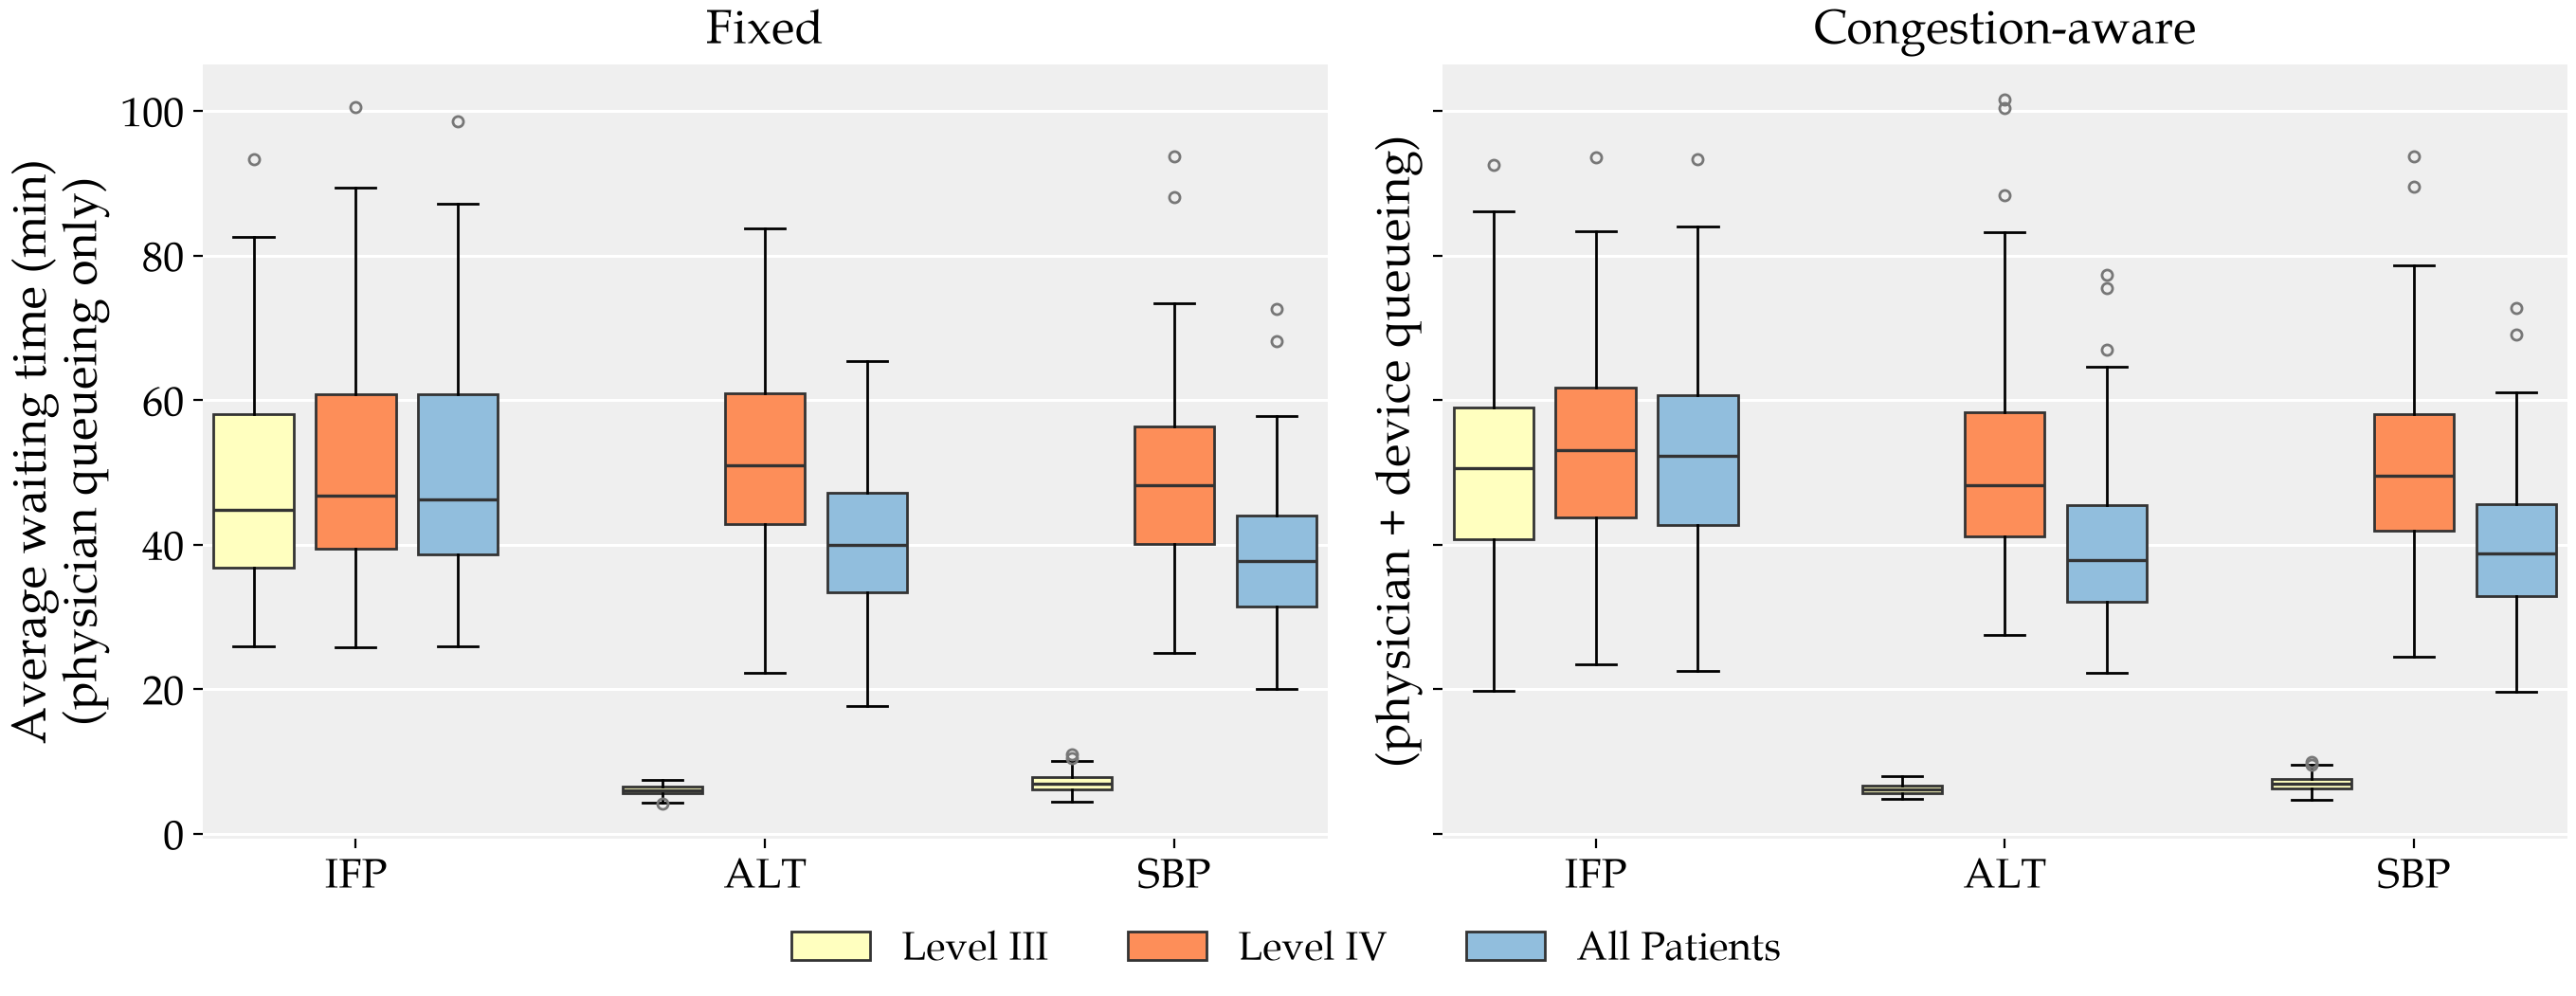
\includegraphics[width=0.96\textwidth]{fig_waiting.png}
\caption{Waiting time by triage level under the three policies: fixed-order
routing (left) and congestion-aware routing (right), $N=100$ replications.
Boxes span the interquartile range and whiskers the remaining spread.}
\label{fig:waiting}
\end{figure*}

\subsection{Effect of the routing rule on the diagnostic stage}
\label{sec:mechanism}

The previous section left one point unexplained: congestion-aware routing
returns patients to the follow-up stage \emph{later}, which is the opposite of
what the rule was designed to do. To isolate the routing rule we run both
diagnostic models under SBP with the same thresholds $(3.3,9.0)$, so that the
examination order is the only difference.

On the quantity it targets, the rule works. Mean station queueing falls from
$0.509$ to $0.365$ min per examined patient, a reduction of $28.2\%$
($t=-18.61$, $p<10^{-30}$). The saving grows with the number of tests a patient
needs (Table~\ref{tab:sojourn}): a patient with one examination sees no
significant change, since there is no ordering decision to make ($p=0.08$),
while a patient requiring all four saves $52\%$. Patients needing all four are
only $3.2\%$ of those examined, so the largest savings accrue to the smallest
group.

The stage as a whole nevertheless takes longer, rising from $29.94$ to $31.44$
min, an increase of $5.0\%$ ($t=49.31$, $p<10^{-60}$). This loss also grows with
the number of tests: $1.04$ min at two, $3.59$ min at three and $6.84$ min at
four. Across all examined patients the rule saves $0.14$ min at the stations
and adds $1.50$ min overall, so every minute saved in a queue costs roughly ten
minutes elsewhere in the stage. The 90th percentile rises from $36.4$ to $40.2$
min, so the loss falls hardest on the patients whose diagnostic stage is
already longest.

\begin{table}[t]
\caption{Station queueing time and total diagnostic-stage time by the number of
examinations a patient requires, $N=100$ replications under SBP with
$(k_1,k_2)=(3.3,9.0)$ in both columns. The last column gives the share of
examined patients. All differences are significant at $p<0.001$ except for
patients requiring a single examination ($p=0.08$ and $p=0.68$).}
\label{tab:sojourn}
\small
\setlength{\tabcolsep}{4pt}
\begin{tabular}{@{}lrrrrr@{}}
\toprule
& \multicolumn{2}{c}{Station queueing (min)} &
\multicolumn{2}{c}{Total stage time (min)} & \\
\cmidrule(lr){2-3}\cmidrule(lr){4-5}
Tests & Fixed & C-aware & Fixed & C-aware & Share \\
\midrule
1 & $0.163$ & $0.156$ & $22.54$ & $22.53$ & $28.7\%$ \\
2 & $0.473$ & $0.392$ & $31.54$ & $32.59$ & $46.0\%$ \\
3 & $0.911$ & $0.538$ & $35.16$ & $38.75$ & $22.1\%$ \\
4 & $1.341$ & $0.643$ & $36.99$ & $43.82$ & $3.2\%$ \\
\midrule
Mean / Total & $0.509$ & $\mathbf{0.365}$ & $29.94$ & $\mathbf{31.44}$ & $100\%$ \\
& \multicolumn{2}{c}{$-28.2\%$} & \multicolumn{2}{c}{$+5.0\%$} & \\
\bottomrule
\end{tabular}
\end{table}

The ratio follows from the relative size of the two quantities. Station
queueing is only $1.70\%$ of the diagnostic stage ($0.509/29.94$), which is
what stations at $14$--$19\%$ utilization (Table~\ref{tab:devices}) would give.
The remaining $98.3\%$ is dominated by reporting delays. The rule therefore
competes for a small share of the stage, while the order it chooses decides how
much of the large share elapses in parallel.

That second effect is where the time goes. A report is prepared while the
patient is already at the next station, so the examination order determines how
much of this waiting overlaps. Consider a patient requiring laboratory, CT and
X-ray. Ordering by descending $\delta_j$ starts with X-ray, and its $30$-minute
report is prepared during the CT and laboratory examinations.
Rule~(\ref{eq:rule}) never reads $\delta_j$: it starts with the $1.19$-minute
laboratory test because that station has the smallest expected workload, and
can leave the $30$-minute X-ray report until last, with no remaining
examination to run alongside it. Since $71.3\%$ of examined patients require two
or more examinations, this situation is common rather than exceptional.

The lesson generalizes beyond this model. A local rule that improves a
congestion signal it can observe may still make the system worse when that
signal is a small part of the delay it is meant to reduce. Decomposing the
diagnostic stage as in Table~\ref{tab:sojourn} would have revealed this before
the rule was implemented.

\subsection{Transferability of tuned thresholds}
\label{sec:transfer}

Section~\ref{sec:mechanism} held the SBP thresholds fixed. They need not be.
Tuning SBP separately for each diagnostic model gives substantially different
answers, $(3.3,9.0)$ against $(12.0,24.0)$ --- the Level III anticipation
margin is almost four times wider in the second case. This means the SBP
columns of Table~\ref{tab:main} differ in two ways at once, so the separate
contributions of the routing rule and the thresholds cannot be read from that
comparison. To separate them we evaluate all four combinations of diagnostic
model and threshold pair on the same $100$ seeds (Table~\ref{tab:transfer}).

\begin{table}[t]
\caption{SBP threshold transfer. Upper block: mean total waiting time for each
combination of diagnostic model and threshold pair. Lower block: the change
from the fixed-order model at its own thresholds, with paired $t$-tests against
that combination, $N=100$.}
\label{tab:transfer}
\small
\setlength{\tabcolsep}{4pt}
\begin{tabular}{@{}lrrr@{}}
\toprule
$\Wtot$ (min) & \multicolumn{2}{r}{$(3.3,9.0)$} & $(12.0,24.0)$ \\
\midrule
Fixed order       & \multicolumn{2}{r}{$\mathbf{38.33}$} & $41.08$ \\
Congestion-aware  & \multicolumn{2}{r}{$42.78$} & $\mathbf{39.08}$ \\
\midrule
\textit{Decomposition} & $\Delta\Wtot$ (min) & $t$ & $p$ \\
Change the routing rule only & $+4.45$ & $3.06$ & $0.003$ \\
Change the thresholds only   & $+2.75$ & $1.89$ & $0.062$ \\
Change both                  & $+0.74$ & $0.54$ & $0.59$ \\
\bottomrule
\end{tabular}
\end{table}

In each row the threshold pair tuned for that model gives the lower waiting
time, so neither pair is suitable for both. Starting from the fixed order at
its own thresholds ($38.33$ min), each change on its own is a loss. Adopting
congestion-aware routing while keeping the old thresholds costs $4.45$ min
($p=0.003$), of which about $0.3$ min is the station queueing that the
fixed-order measure does not count. Adopting the new thresholds under the old
routing rule costs $2.75$ min. Making both changes together costs $0.74$ min,
which is not significant ($p=0.59$).

The two losses therefore do not add: separately they come to roughly $7$ min,
together to less than one. Each change is harmful without the other and
harmless with it, so the diagnostic routing rule and the scheduling thresholds
behave as a pair rather than as two independent design choices. In practical
terms, a department adopting a new diagnostic process should re-tune its
scheduling policy at the same time, since adopting one without the other is
worse than adopting neither.

The same decomposition also guards against a misreading of the service level.
Between the two tuned configurations, SBP's Level III service level rises from
$97.32\%$ to $99.95\%$ (Table~\ref{tab:sl}), which invites the conclusion that
congestion-aware routing protects urgent patients. It does not. The new
thresholds account for $+2.63$ percentage points ($t=-18.54$, $p<0.001$), while
the routing rule on its own costs $0.48$ points ($t=2.59$, $p=0.011$). A study
reporting only the two tuned configurations would credit the gain to the wrong
change and report the routing rule's effect with the wrong sign.

\subsection{Sensitivity to demand and staffing}
\label{sec:robustness}

The preceding experiments use the arrival rates and staffing
of~\cite{lv2026des}. We now vary the arrival rate by $\pm15\%$ in $3\%$
increments and physician staffing over seven scenarios from $5/5/3$ to $7/7/5$
(Figures~\ref{fig:arrival} and~\ref{fig:staffing}). Each point uses $20$
replications on a separate seed stream, one fifth of what the earlier sections
use, so we read these sweeps as trends rather than as values.

\begin{figure*}[t]
\centering
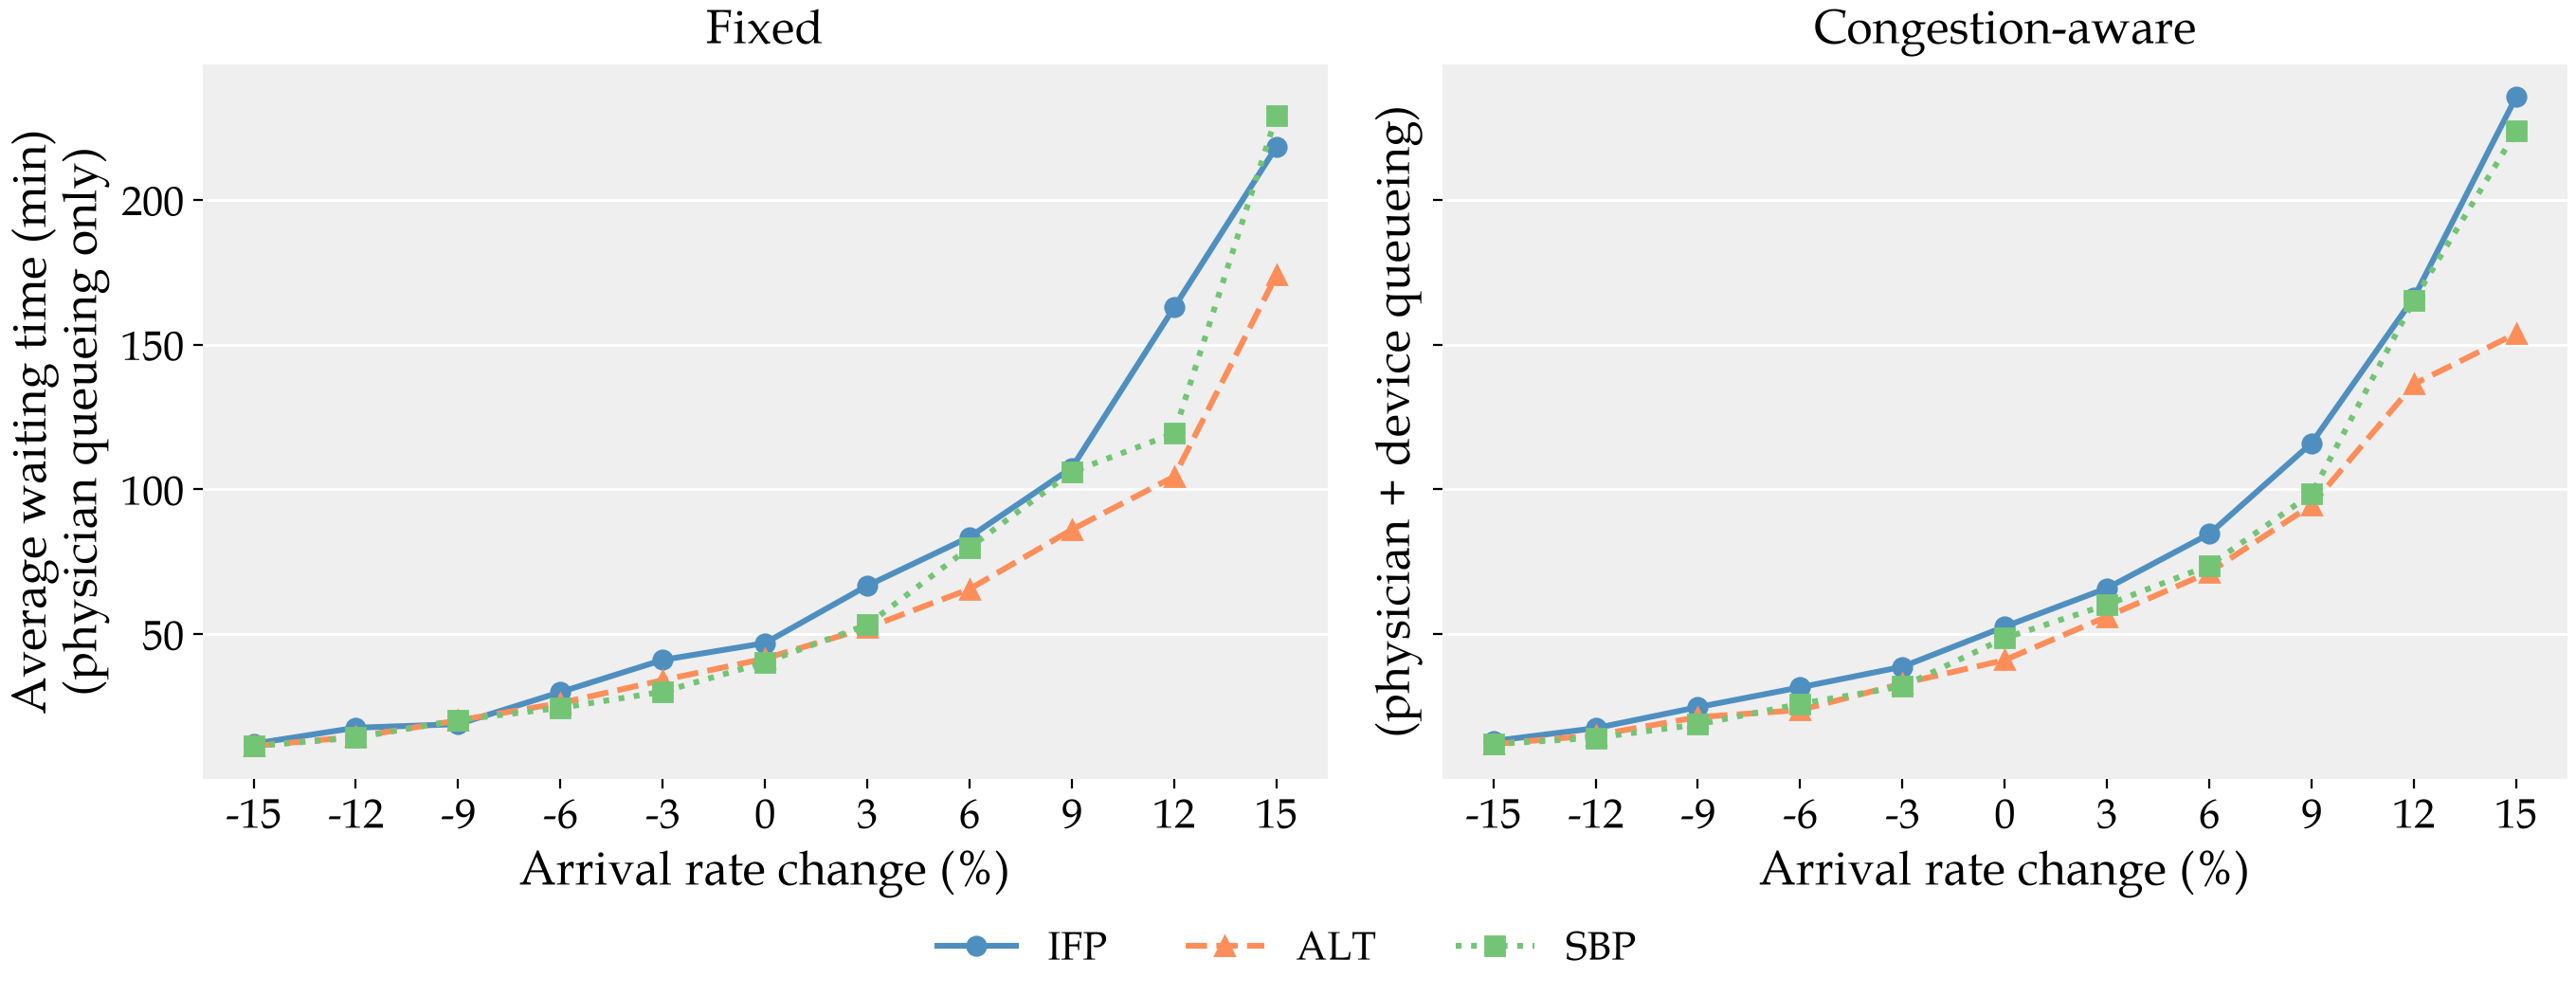
\includegraphics[width=0.96\textwidth]{fig_arrival.png}
\caption{Mean waiting time as the arrival rate varies by $\pm15\%$ around the
rates of~\cite{lv2026des}, $20$ replications per point.}
\label{fig:arrival}
\end{figure*}

\begin{figure*}[t]
\centering
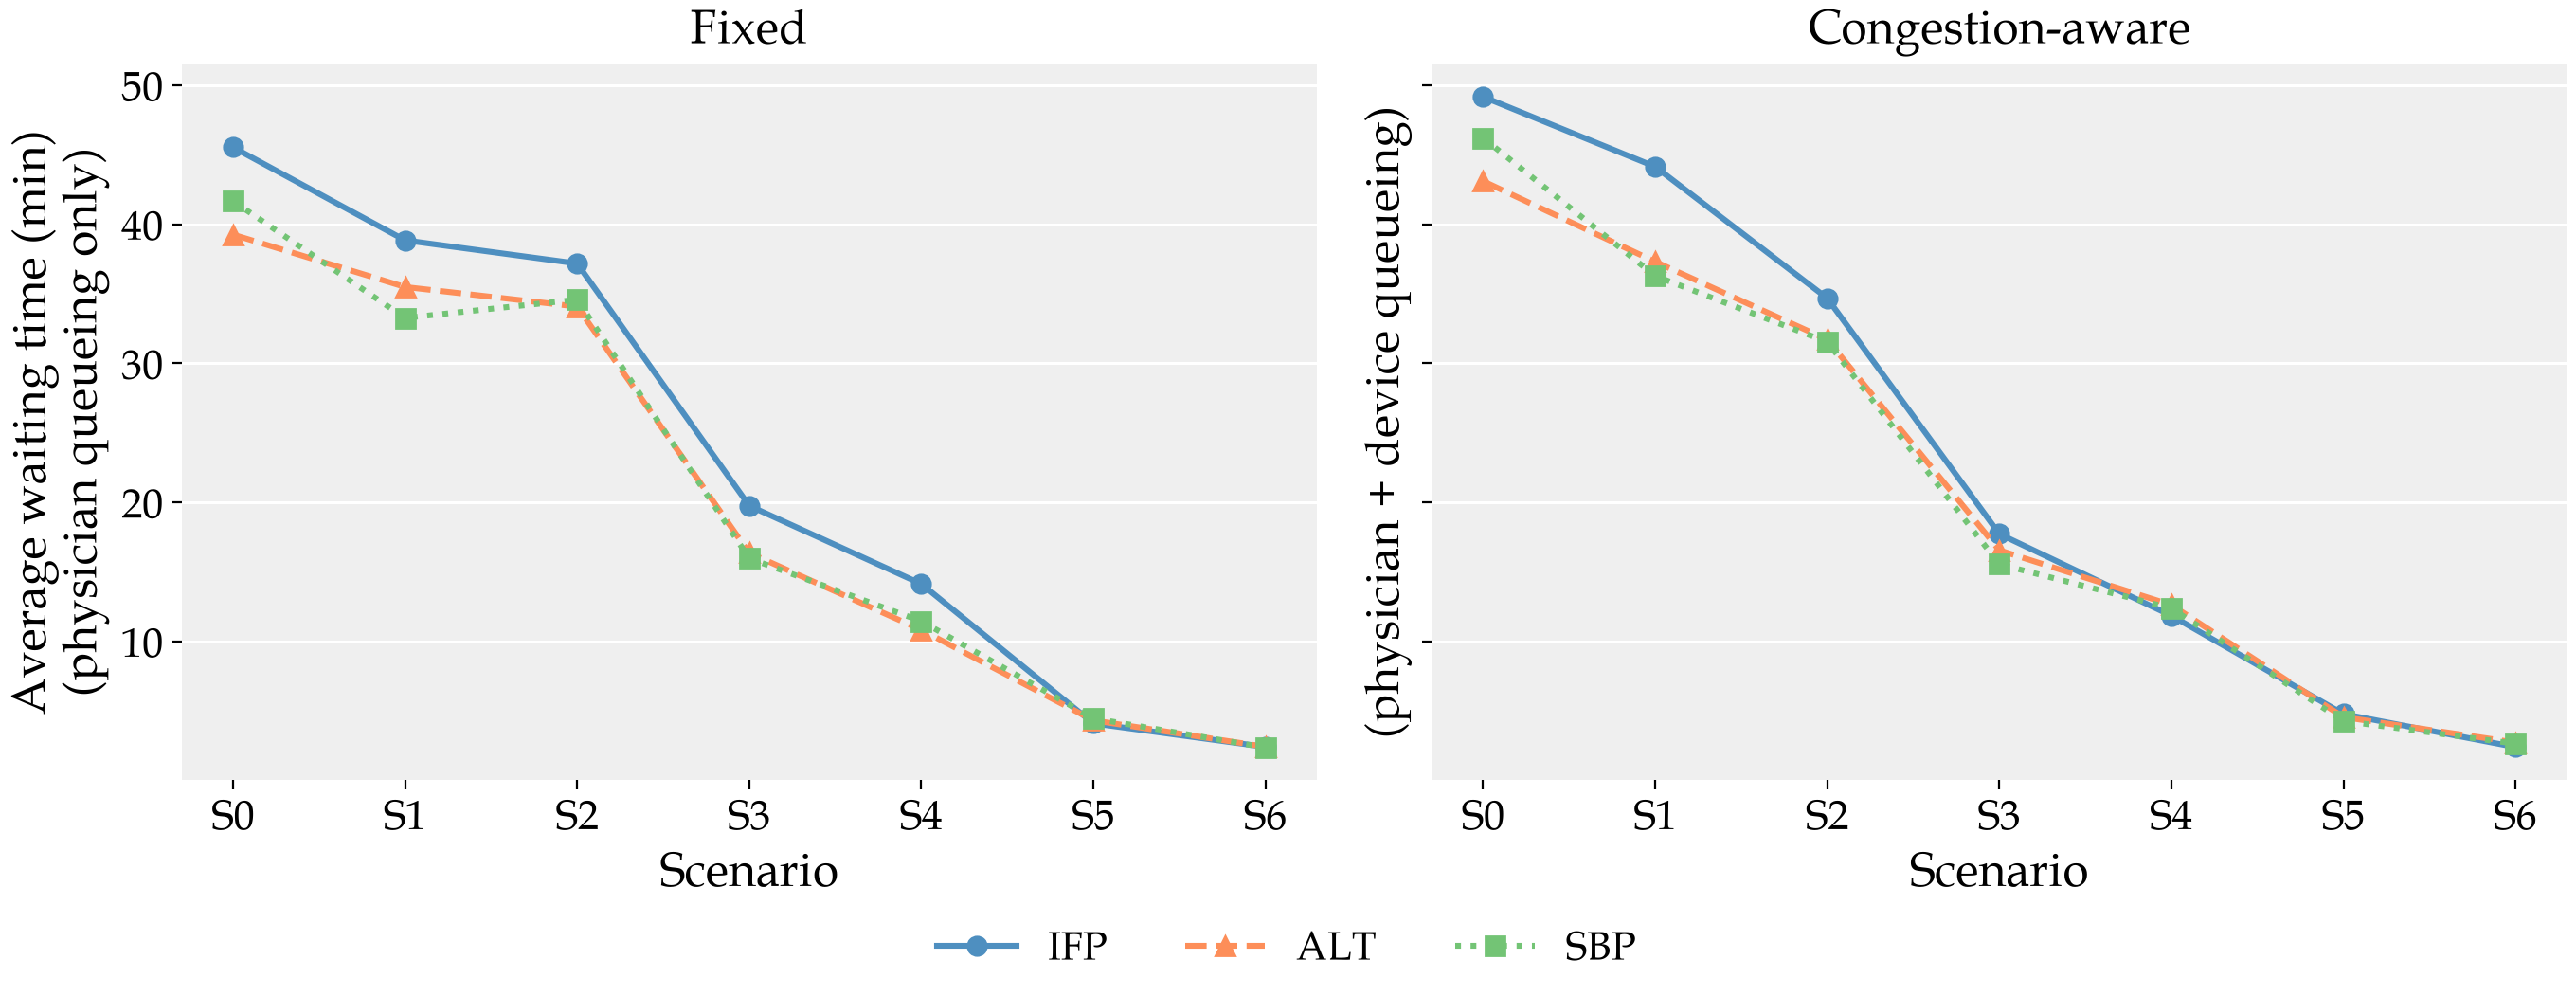
\includegraphics[width=0.96\textwidth]{fig_staffing.png}
\caption{Mean waiting time across staffing scenarios S0 ($5/5/3$) to S6
($7/7/5$), $20$ replications per point.}
\label{fig:staffing}
\end{figure*}

The first trend concerns SBP. Its advantage over ALT does not survive added
demand: from $+3\%$ onward ALT gives the lower mean waiting time under both
diagnostic models, and the gap widens with load. At $+15\%$ ALT averages $174$
min against $229$ min for SBP under the fixed order, where SBP is by then
slower than IFP as well, and $154$ against $224$ min under congestion-aware
routing. The reason lies in the rule itself. SBP serves whoever is closest to
breaching their target, which discriminates usefully only while most patients
remain inside their target; once nearly everyone is late, the rule has little
left to distinguish between them. ALT never evaluates urgency and continues to
direct a fixed share of capacity to the follow-up queue regardless of load.
This does not support the conclusion of~\cite{lv2026des} that the slack-based
policy performs best across operating conditions, and the disagreement falls
exactly on the conditions under which the choice of policy matters most.

The second trend concerns the physicians. The seven scenarios progressively add
physicians across the three shifts: S0$=5/5/3$, S1$=5/5/4$, S2$=5/5/5$,
S3$=5/6/5$, S4$=5/7/5$, S5$=6/7/5$, S6$=7/7/5$. All three policies fall below
$20$ min of mean waiting time by S3, and by S5 they lie within $0.4$ min of
each other under the fixed order and $0.5$ min under congestion-aware routing.
Once physicians are no longer scarce, how they are allocated stops mattering,
which is the same conclusion Section~\ref{sec:mechanism} reached from the
opposite direction: the physicians are the binding resource, not the stations.
Physician utilization is approximately $86\%$ against $14$--$19\%$ at the
stations, so additional imaging capacity would change little.

Neither sweep settles the effect of the routing rule itself: at $20$
replications per point it moves some points up and others down with no
consistent direction, which is why that question was answered in
Section~\ref{sec:transfer} instead. Nor does either sweep put pressure on the
stations, which remain below $20\%$ utilization throughout.


\section{Conclusion and Future Work}
\label{sec:conclusion}

\subsection{Key takeaways}

This project reproduced the ED scheduling model of Lv et al.~\cite{lv2026des}
and extended its diagnostic stage to a congestion-aware representation with
per-station queues. Three findings follow.

First, congestion-aware routing reduces station queueing by $28.2\%$ yet
lengthens the diagnostic stage by $5.0\%$, because station queueing is only
$1.70\%$ of that stage while the order the rule discards had been overlapping
the reporting delays that dominate it. Added realism is therefore worth
introducing in proportion to the share of time the modelled component accounts
for, and that share can be established before a rule is designed.

Second, the diagnostic routing rule and the SBP thresholds cannot be changed
one at a time. Each change is harmful in isolation ($+4.45$ and $+2.75$ min)
but approximately neutral together ($+0.74$ min, not significant). The same
decomposition shows that the apparent gain in Level III service level between
the two tuned configurations comes from the thresholds, not from the routing
rule, which works against it.

Third, the ranking of policies reported in the base paper does not hold under
stress. From only $+3\%$ additional demand, the parameter-free alternating
policy overtakes the tuned slack-based policy, and at $+15\%$ the slack-based
policy is slower even than the fixed-priority policy.

\subsection{Limitations}

The model retains several simplifying assumptions. Only Level III and IV
patients are represented, so no resuscitation pre-empts a consultation. Each
modality has one server, inferred from the reported equipment availability
rather than stated. All required examinations are known before testing begins,
so a result that triggers a further test --- common in practice, and the case
that would stress our rule most --- is not modelled. Physicians are
interchangeable, and nothing downstream such as ward-bed availability backs up
into the department. The service-level bound $SL^{\min}_\ell=0.90$ in
(\ref{eq:opt}) is a modelling choice that directly affects the optimized
thresholds, and the SBP waiting clock runs from arrival rather than resetting
at the follow-up queue.

Methodologically, each replication starts from an empty system with no warm-up,
which pulls early waiting times down by an unknown amount; a Welch
procedure~\cite{welch1983warmup} would remove this. Although seeds are reused
for paired comparisons, two policies given the same seed draw random numbers in
a different order and diverge within a few events, so the variance reduction is
small; separate random streams per process would give stronger
common-random-number control~\cite{law2015simulation}. The staffing sweep only
adds physicians and never removes them, so reduced staffing is untested.

\subsection{Future work}

Three directions follow directly from these results. The first is a routing
score that carries both signals, for instance $n_j(t)\tau_j-\delta_j$, which
would begin with the longest-reporting examination, as the fixed order does,
and let congestion break ties only among examinations whose reports arrive at
about the same time. The second is joint rather than sequential optimization of
the routing rule and the scheduling thresholds, since
Section~\ref{sec:transfer} shows that they behave as a pair. The third is to
establish where congestion-aware routing pays off: the stations here never
exceed $20\%$ utilization, and a department with fewer machines, longer
examinations or a higher testing rate would give the rule a signal large enough
to work with. The grid search is also worth replacing, since the top five
fine-grid candidates lie within $1.04$ min of each other and a derivative-free
method would reach them at a fraction of the cost.

\bibliographystyle{ACM-Reference-Format}
\bibliography{refs}

\end{document}